\section{Application}\label{sec:Application}
%The main purpose of glyphs is to represent single or multiple data attributes using a geometric primitive.
Glyph-based visualization is an excellent tool for representing single or multiple data attributes.
Whilst generic glyphs are desirable and have been well-studied (e.g., Star glyphs~\cite{siegel72} and Chernoff faces~\cite{Chernoff73faces}), the effectiveness of such designs for conveying information are limited when presented with challenging, complex data forms such as vector and tensor data.
In addition to various data type constraints, other factors must be considered.
For example, the sampling resolution greatly affects how small or how large the glyph can be in order to avoid visual clutter (compare to DG2).
Thus, we find that many glyphs are attribute-dependant and that their specific application context is an integral aspect to the design process. 
%Thus, many glyphs are application or attribute-dependant in which the context they are used is an integral aspect within the design process.
In this section, we report a selection of important papers that focus on novel glyph-based visual techniques that have been explored and utilised in various scientific domains.

\subsection{Medical Visualization}

%Taxonomy and Usage Guidelines for Glyph-based Medical Visualization by
%A comprehensive overview of existing glyph-based visualization techniques used in the medical domain is provided by T. Ropinski and B. Preim~\cite{ropinski08} and describe guidelines for developing more valuable glyph representations.
The recent survey by Ropinski and Preim~\cite{ropinskiPreim08glyphTaxonomy,Ropinski11glyphs} provides an overview of existing glyph-based visualization techniques used in the medical domain and propose guidelines for developing more valuable glyph representations. 
A glyph taxonomy based on the way information is processed when interpreting glyph visualizations is used to classify such techniques.
Within semiotic theory, this consists of a two-phase information process:
%Based on semiotic theory, glyph-techniques are categorised into the following classification: 
%In particular, the authors focus on using the following classification as described in semiotic theory: 
1) \textit{pre-attentive} processing, that is mainly stimulated by glyph attributes such as size, colour and shape along with glyph placement, texture mapping and glyph filtering and 2) \textit{attentive stimuli} processes which are based on glyph-interaction paradigms. Examples include a colour legend which users can use to formulate more quantitative glyphs and repositioning glyphs where the glyph properties adapt depending on the location. Based on this classification, the authors describe eight usage guidelines which they evaluate against modern diffusion tensor imaging and cardiac visualization. 

%\begin{figure}[t]
%\centering
%	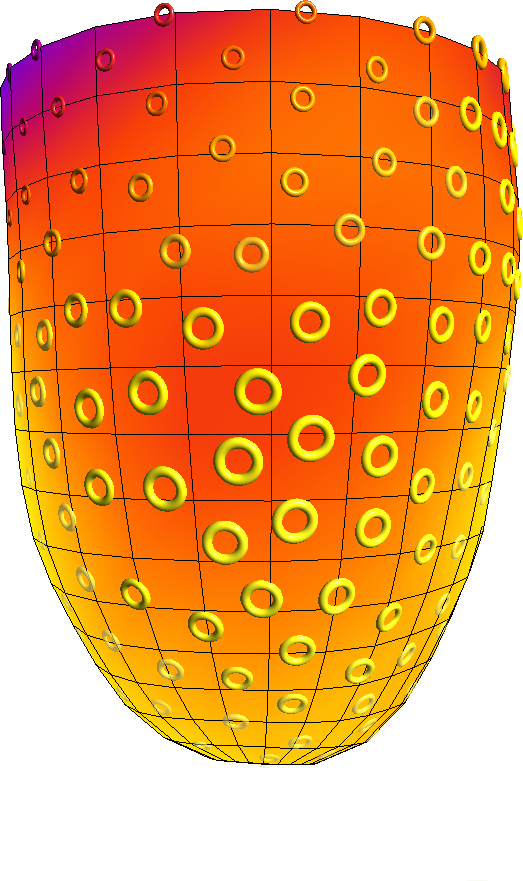
\includegraphics[width = 4cm]{meyerGlyphVis}
%\vspace*{-8mm}
%\caption{Visualization of stress-induced ischemia of the anterolateral wall using 3D glyphs by Meyer-Spradow et al.~\cite{meyer-spradow08glyphSPECT}}
%\label{fig:meyerGlyphVis}
%\end{figure}

%Tensor applications in the medical field
%Processing and visualization for diffusion tensor MRI by 
Westin et al.~\cite{westin02processing} introduce a novel analytical solution to the Stejskal-Tanner diffusion equation system from which a set of derived diffusion tensor metrics describes the geometric properties of a diffusion ellipsoid. Using three tensor eigenvalues, the quantitative shape measures, $c_l, c_p$, and $c_s$ indicate the linear, planar and spherical properties of a tensor.
In addition, the authors present a visualization technique using a composite tensor glyph built from a sphere, disc and rod that are mapped to the three eigenvalues which aims to reduce the ambiguity caused by traditional ellipsoid representation. The composite glyphs are colour-coded according to shape such that blue is mapped to linear case, yellow to planarity and red for spherical case.

%Glyph-Based Visualization of Myocardial Perfusion Data and Enhancement with Contracility and Viability Information by 
Oeltze et. al~\cite{oeltze08myocardial} incorporate 3D glyphs for visualizing  perfusion parameters in conjunction with their ventricular anatomical context. They propose two glyph designs: (a) 3D Bull's Eye Plot (BEP) Segment and (b) 3D Time-Intensity Curve (TIC) Miniatures for depicting four perfusion parameters: \emph{Peak Enhancement (PE)}, \emph{Time To Peak (TTP)}, \emph{Integral} and \emph{Up-slope} which describe the myocardial contractility and viability.
The 3D BEP segments are ring-shaped glyphs which extend the previous work \cite{cerqueira02} from 2D to 3D space.
An improved glyph (TIC miniatures) enables intuitive mapping of all important parameters in cardiac diagnosis as a result of encoding TIC semantic metaphors (glyph shape) that is familiar to domain experts.
They apply their technique on three datasets from a clinical study.

%Glyph-Based SPECT Visualization for the Diagnosis of Coronary Artery Disease by 
The work by Meyer-Spradow et al.~\cite{meyer-spradow08specGlyphs} present an interactive 3D glyph-based approach for the visualization of SPECT-based myocardial perfusion data. They utilise a supertorus prototype glyph which characterises SPECT data based on its colour, opacity, size and roundness. 
%The glyphs is positioned along a 3D surface (i.e., the myocardium) in order to depict the state of the underlying tissue.
The glyphs are positioned along a 3D surface (i.e., the myocardium) using a random distribution with relaxation for depicting information of the underlying tissue. 
One motivation of such a placement strategy is to provide a more even-distribution of glyphs. 
This addresses the problem of unbalanced placement that can occur from regular grid sampling in complex and non-uniform meshes (compare to DG11).

\subsection{Event Visualization}

%In particular, we present a framework for hierarchical event representation, and an importance-based selection algorithm for supporting the creation of a video storyboard from a video. 
%We consider the storyboard to be an event summarization for the whole video, whilst each individual illustration on the board is also an event summarization but for a smaller time window. 
%We utilized a 3D visualization template for depicting and annotating events in illustrations. To demonstrate the concepts and algorithms developed, we use Snooker video visualization as a case study, because it has a concrete and agreeable set of semantic definitions for events and can make 
%use of existing techniques of event detection and 3D reconstruction in a reliable manner. 
%Nevertheless, most of our concepts and algorithms developed for challenges (b) and (c) can be applied to other application areas. 

%Action-based Multifield Video Visualization by
Event and activity visualization is a rapidly growing research topic. 
The work by Botchen et al.~\cite{botchen08ActionBasedVideo} describe the VideoPerpetuoGram (VPG), a dynamic technique for visualizing activity recognition found in video streams. This involves stacking temporally spaced intervals of key video frames and using colour filled glyphs to represent geometric information (e.g., object identifier, position, size), semantic information (e.g., action type and inter-object relation) and statistical information (the certainty and error margins of the analytical results). They demonstrate their technique on surveillance video footage for summarizing the motion of people and actions.

%Visualizing network security events using compound glyphs from a service-oriented perspective by 
Pearlman and Rheingans~\cite{pearlman08securityEvent} introduce a glyph-based approach for visualizing computer network security using compound glyphs. The compound glyph representation is a pie chart in which the size and colour of each segment is mapped to the amount of activity and the type of service.
One of the motivations of using a simple pie chart design, is its ability to extend to the temporal domain by slicing the glyph as concentric layers for depicting information at different time instances.
Each glyph indicates a node on the network in which connectivity lines in the visualization represent the communication between nodes.
They successfully demonstrate their method on a simulated network consisting of a small set client users.

%Video Visualization for Snooker Skill Training by 
%H\"{o}ferlin \textit{et al.}~\cite{hoferlin10} presents a feasibility study on using video visualization to aid snooker skill training. By involving the coaches and players in the loop of intelligent reasoning, their approach addresses the difficulties of automated semantic reasoning, while benefiting from mature video processing techniques. 
%In particular, they utilise the principal design of the VideoPerpetuoGram (VPG) to convey spatiotemporal information to the viewers through static visualization, removing the burden of repeated video viewing. 
%We extended the VPG design to accommodate the need for depicting multiple video streams and respective temporal attribute fields, including silhouette extrusion, spatial attributes, and non-spatial attributes. 
%Our results and evaluation have shown that video visualization can provide snooker coaching with visually quantifiable and comparable summary records, and is thus a cost-effective means for assessing skill levels and monitoring progress objectively and consistently. 

The work by Parry et al.~\cite{parry11} introduce a novel event selection concept for summarising video storyboards. Video storyboard is a form of video visualization, used to summarise the major events in a video using illustrative visualization.
There are three main technical challenges in creating a video storyboard, (a) event classification, (b) event selection and 
(c) event illustration. Among these challenges, (a) is highly application-dependent and requires a significant amount of application- 
specific semantics to be encoded in this system or manually specified by the users. 
This paper focuses on challenges (b) and (c) which they demonstrate using a case study on Snooker video visualization. 
For event illustration, the authors explore a collection of iconic glyphs which convey some metaphors in addition to data values for event labelling. 
These include ball objects that vary in size, opacity and colour for representing ball trajectory and semantic information (e.g., ball type, event importance), textured circle glyphs and numbered icons for depicting the sequences of shots, and a pie chart icon to represent scoring and video timing information.

\begin{figure}[t]
\begin{center}
	\subfloat[]{
		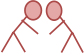
\includegraphics[width = 2cm]{images/related-work-glyphs/stickman_scrum1}
		\label{fig:alt_design_1}
	}
	\subfloat[]{
		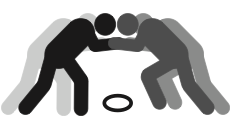
\includegraphics[width = 2.6cm]{images/related-work-glyphs/stickman_scrum2}
		\label{fig:alt_design_2}
	}
	\subfloat[]{
		
\includegraphics[height = 2cm]{images/related-work-glyphs/contemporary_player}
		\label{fig:alt_design_3}
	}
	\\
	\vspace*{-2mm}
	\subfloat[]{
		
\includegraphics[height = 2cm]{images/related-work-glyphs/posterize_player}
		\label{fig:alt_design_4}
	}
	\subfloat[]{
		
\includegraphics[height = 2cm]{images/related-work-glyphs/silohette_player}
		\label{fig:alt_design_5}
	}
	\subfloat[]{
		
\includegraphics[width = 2.6cm]{images/related-work-glyphs/silohette_scrum}
		\label{fig:alt_design_6}
	}
\end{center}
\caption{Some designs of metaphoric pictograms for visualizing event data in Rugby by Legg et al.~\cite{legg12matchPad}. In (a), initial stickmen designs were produced to prompt an artist. The artist produced several different designs: (b) a refined stickman design, (c) contemporary design, (d) a posterised colour design and (e) a silhouette design. In (f) the scrum is depicted using the silhouette design (cf. (a) and (b))}
\label{fig:metaphoricPictograms}
\end{figure}

%Different glyph design options prove to be more effective by exploring the full extent of the data space given an application context.
A more thorough investigation of incorporating visual semantics into glyph designs is explored by Legg et al.~\cite{legg12matchPad}. 
%The work by Legg~\textit{et al.}~\cite{legg12matchPad} demonstrates 
They describe the MatchPad: an interactive glyph-based visualization for mapping events and actions in sports notational analysis. 
Sports event analysis provides an example where a large number of event types need to be depicted in a manner to facilitate rapid information retrieval. 
A comprehensive review of mapping such data is discussed using different levels of abstractions. 
These include the evaluation of abstract icons and colour for encoding each event type.
Whilst the approach may be suitable for data attributes with a small number of enumerative values, the range of categorical attributes in sports results to many different shapes or colours making it cognitively challenging to learn, remember or guess.  
Instead, the authors explore the use of metaphoric pictograms which are commonly used in many domain-specific visualization (e.g., electronic circuit diagrams) and visualization for the masses (e.g., road signs).
Metaphoric glyphs can come in different forms, ranging from abstract representation to photographic icons (Figure~\ref{fig:metaphoricPictograms}), where the use of appropriate visual channels can provide semantic cues that are easy to learn, remember or guess.
The MatchPad adopts a scale-adaptive layout to position glyphs along a timeline interactively based on the viewpoint zoom factor. 
This minimises glyph occlusion which they demonstrate successfully using a case study on Rugby.
%They demonstrate the MatchPad software with a case study on Rugby, which utilises a scale-adaptive layout to position the glyphs along a timeline interactively based on the viewpoint zoom factor to minimise glyph occlusion. 
%The glyph-based visualization uses a scale-adaptive layout to position the glyphs along a timeline interactively, based on the viewpoint zoom factor to minimise glyph occlusion. 
%The authors demonstrate their visualization software, MatchPad, with a case study on rugby event analysis.

\subsection{Multi-field Visualization}

Due to its multivariate characteristics, geometric shapes are commonly used to represent multiple data attributes. Superquadrics and Angle-Preserving Transformations by Barr~\cite{barr81} presents such an approach by introducing geometric shapes (superquadrics) used for creating and simulating three-dimensional scenes. The author defines a mathematical framework used to explicitly define a family of geometric primitives from which their position, size, and surface curvature can be altered by modifying a family of different parameters. Example glyphs include: a torus, star-shape, ellipsoid, hyperboloid, toroid. Furthermore, the author describes angle-preserving shape transformations that can be applied to primitives to create geometric effects such as bending or twisting.

%A Scientific Visualization Synthesizer by 
Crawfis and Allison~\cite{crawfis91} introduce a novel approach for visualizing multiple scientific data sets using texture mapping and raster operations. 
The interactive programming framework enables users to overlay different data sets by defining raster functions/operations. 
Such a function may include glyph textures for mapping data attributes (e.g., vector data).
Using a generated synthetic dataset, they present a method for reducing the visual clutter by mapping colour to a height field and using a bump map to represent the vector and contour plots. The final texture is mapped onto a 3D surface. 

Using the set of superquadrics defined by Barr~\cite{barr81}, Shaw et. al~\cite{shaw98} describe an interactive glyph-based framework for visualizing multi-dimensional data. 
As opposed to the analytical focus in the previous work, the authors describe a method for mapping data attributes appropriately to shape properties such that visual cues effectively convey data dimensionality without depreciating the cognition of global data patterns. They map in decreasing order of data importance, values to location, size, colour and shape (of which two dimensions are encoded by shape). Using superellipsoids, they apply their framework to the "thematic" document similarities \cite{shaw98} and magnetohydrodynamics simulation of the solar wind in the distant heliosphere \cite{ebert00}, \cite{ebert01}.

%Visualizing Multiple Fields on the Same Surface by 
The report by Taylor~\cite{taylor02} provides an overview of successful and unsuccessful techniques for visualizing multiple scalar fields on a 2D manifold. 
The author first hypothesises that the largest number of data sets can be displayed by mapping each field to the following: a unique surface characteristic, applying a different visualization technique to each scalar field or by using textures/glyphs whose features depend on the data sets. Such a framework revealed limitations of up to four scalar fields.
This led to the research of two new techniques that prove effective for visualizing multiple scalar fields, (1) \emph{data-driven spots (DDS)}~\cite{bokinsky03dataDrivenSpots} - using different spots of various intensities and heights to visualize each data set, and (2) \emph{oriented slivers}~\cite{weigle00orientedSlivers} - using sliver-like texture glyphs of different orientations for visualizing multiple scalar fields in which luminance is mapped to the relative scalar values.

One successful technique is developed by Kirby and Laidlaw~\cite{kirby99multiValueFlow} who stochastically arrange multiple visualization layers to minimize overlap. 
This paper extends the work by Laidlaw et. al~\cite{laidlaw98} by applying visualization concepts from oil painting, art and design, to the problems in fluid mechanics.
Given a permutation of layers, a user-specified importance value is attached to each visualization of increasing weights in order to provide greater emphasis to higher layers.
Visual cues such as colour and opacity indicate regions and layers of importance (e.g., Rate of strain tensor example emphasise the velocity more by using black arrows). 
This method enables the simultaneous depiction of 6-9 data attributes, in which the authors apply to a simulated 2D flow field past a cylinder at different reynolds number. 
The example shows the visualization of velocity, vorticity, rate of strain tensor, turbulent charge and turbulent current using a series of visualization techniques such as tensor ellipses, vector arrows and colour mapping.  

%Oriented Sliver Textures: A Technique for Local Value Estimation of Multiple Scalar Fields by Weigle et al.~\cite{weigle00orientedSlivers} describe the use of glyph-like textures (slivers) for visualizing multiple scalar fields. The authors depict each field as a texture slivers of different degrees of orientation in which luminance is mapped to their relative scalar values. In the final step, each scalar representation is overlayed into a single image for simultaneous viewing. The authors demonstrate their work on a scanning electron microscope (SEM) data set containing 8 different scalar fields.

\subsection{Geo-spatial Visualization}

We often find that geo-spatial visualization may incorporate inter-disciplinary techniques from other domains, and thus can be classified under more than one category. MacEachren et al.~\cite{maceachren98visualizingGeoreferenced} is such an example where the authors present a novel approach to visualize reliability in mortality maps using a bi-variate mapping. Given a base geographical map (United States), the technique involves using colour filled regions to represent the data and texture overlay to represent the reliability.

%Large Datasets at a Glance: Combining Textures and colours in Scientific Visualization by 
Healey and Enns introduce a different approach~\cite{healey99largeDatasetsAtGlance} using multi-coloured perceptual texture elements known as \textit{pexels} for visualizing multivariate scientific datasets across a height field. The pexels appearance is determined by encoding attribute values into three texture dimensions: height, density and regularity.
Pexels incorporate pre-attentive features (e.g., height) to improve the accuracy of visual search-based tasks.
To assess its effectiveness, the authors apply their technique on a typhoon data set where wind speed, pressure and precipitation is mapped to the pexel properties.

Pang~\cite{pang01uncertaintyGeospatial} provides an overview of various geo-spatial uncertainty metrics and identifies two methods for integrating this data into a geo-spatial representation: (a) mapping uncertainty information to graphic attributes (e.g., hue, opacity) or by using (b) animation to convey uncertainty.
By treating uncertainty fields as an additional layer of information in cartography, techniques such as uncertainty glyphs can be visualised independently and overlaid on top of an existing geo-spatial visualization.

%Noodles: A Tool for Visualization of Numerical Weather Model Ensemble Uncertainty by 
The work of Sanyal et al.~\cite{sanyal10} introduce glyphs, ribbons and spaghetti plots for interactively visualizing ensemble uncertainty in numerical weather models. They demonstrate their work on the 1933 Superstorm simulation, where the visual mappings illustrate the statistical errors (e.g., mean, standard deviation, interquartile range and 95\% confidence intervals) in the data.

\subsection{Flow Visualization}

%In the flow visualization community, De Leeuw and Van Wijk~\cite{deLeeuwVanWijk93probe} visualize the local properties of a flow field by visualizing its gradient (Jacobian). They decompose the Jacobian matrix into symmetrical and anti-symmetrical constituents which are transformed to a local coordinate frame and further decomposed into different components representing acceleration, shear, curvature, torsion, and convergence, respectively. These components can then be mapped to different geometric primitives for visualization.

In the flow visualization community, De Leeuw and Van Wijk~~\cite{deLeeuwVanWijk93probe} present an interactive probe-glyph for visualizing multiple flow characteristics in a small region.
One focus is the visualization of six components: velocity, curvature, shear, acceleration, torsion and convergence.
In order to facilitate such a mapping, the authors incorporate a larger glyph design.
The core components of the glyph consists of the following: 1) a curved vector arrow where the length and direction represents the velocity and the curvedness is mapped to the curvature, 2) a membrane perpendicular to the flow where its displacement to the centre is mapped to acceleration, 3) candy stripes on the surface of the velocity arrow illustrates the amount of torsion, 4) a ring describes the plane perpendicular to the flow over time (shear-plane), and finally 5) the convergence and divergence of the flow is mapped to a \emph{lens} or osculating paraboloid. Placement of such probes are interactively placed by the users along a streamline to show local features in more detail. 

\begin{figure}[t]
\centering
	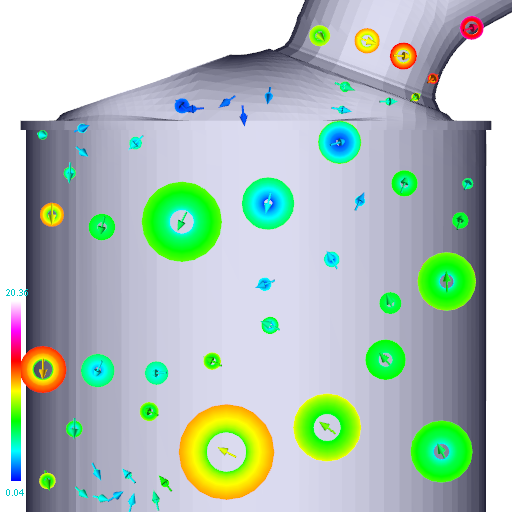
\includegraphics[width = 6cm]{images/related-work-glyphs/peng12compositeGlyph}
\caption{The visualization of vector field clustering of flow around an engine. A combination of $|v|$-range and $\theta$-range glyph is used for depicting the range of vector magnitude and direction in each vector cluster~\cite{peng12meshDriven}}
\label{fig:engineFlowGlyph}
\end{figure}

Vector Plots for Irregular Grids Dovey~\cite{dovey95} extends Crawfis and Max's method~\cite{crawfisMax92} from regular to curvilinear and unstructured grids. In order to visualize vector fields on unstructured grids, physical space and parameter space resampling methods are employed. 
During the physical space resampling, the vector field is linearly interpolated at each sample point, then the physical coordinates of the point are calculated, and lastly related oriented glyphs (plots) are projected from back to front. 
Although this ensures that sample points are uniformly distributed, physical space resampling is computationally expensive. To address this problem, it may be preferable to resample to parameter space instead. 
At first, random points are directly generated in parametric space with an area-weighted distribution. Then a relatively accurate and dense resampling can be approximated by mapping the parameterised coordinate to physical coordinate grid points. Vector field visualization on arbitrary 3D surfaces can be efficiently achieved with parameter space resampling. 

%Higher Dimensional Vector Field Visualization: A Survey by Peng \textit{et al.}~\cite{peng11}: Vector field visualization research has evolved very rapidly over the last two decades. There is growing consensus amongst the research community that the challenge of two-dimensional vector field visualization is virtually solved as a result of the tremendous amount of effort put into this problem. 
%Two-dimensional flow, both steady and unsteady can be visualized in real-time, with complete coverage of the flow without much difficulty. 
%However, the same cannot be said of flow in higher-spatial dimensions, e.g. surfaces in 3D (2.5D) or volumetric flow (3D). 
%We present a survey of higher-spatial dimensional flow visualization techniques based on the presumption that little work remains for the case of two dimensional flow whereas many challenges still remain for the cases of 2.5D and 3D domains. This survey provides the most up-to-date review of the state-of-the-art of flow visualization in higher dimensions. The reader is provided with a high-level overview of research in the field highlighting both solved and unsolved problems in this rapidly evolving direction of research. 

%Result of a User Study on 2D Hurricane Visualization by 
Martin et al.~\cite{martin08hurricaneUserStudy} present a study to validate the effectiveness of traditional 2D hurricane visualizations by observing the users ability to mentally integrate the magnitude and direction of flow in a vector field. In particular, the authors focus on evaluating 2D glyphs (or wind barb) - a technique commonly used for depicting wind magnitude and direction in weather visualizations. For both magnitude and direction, users had to estimate the value at a given point and estimate the average value over a rectangular region. The authors use a real hurricane simulation data set in their study.

%Flow Radar Glyphs - Static Visualization of Unsteady Flow with Uncertainty by 
Hlawatsch et al.~\cite{hlawatsch11flowRadar} introduce a glyph for visualizing unsteady flow with static images. The flow-radar (glyph) is constructed by transforming time-dependant vector attributes into polar co-ordinates, whereby vector direction is mapped to angle, and the time to radius. In addition, the velocity magnitude is encoded using colour. The radar glyphs provides a visual summary of the flow over multiple time steps. A method for visualizing flow uncertainty is described using a single arc that represents the angular variation at given seed point. The authors demonstrate their work on two CFD simulation data set.

Peng et al.~\cite{peng12meshDriven} describe an automatic vector field clustering algorithm and presents visualization techniques that incorporate statistical-based multivariate glyphs. The authors clustering algorithm is given by: 1) derive a mesh resolution value for each vertex, 2) encode vector and mesh resolution values into R, G, B and $\alpha$ in image space. Clusters naturally form in this space based on pixel intensity. 3) the clusters are merged depending on a similarity value derived using euclidean distance, mesh resolution, average velocity magnitude and velocity direction. A collection of clustering glyph-based visualizations are introduced, such as $|v|$-range glyph or ``disc'' (Figure~\ref{fig:engineFlowGlyph} for example) that depicts the local minimum and maximum vector. The inner and outer radius of the disc is mapped to the vector magnitudes. The $\theta$-range glyph combines a vector glyph that illustrates the average velocity direction and magnitude, and a semi-transparent cone that shows the variance of vector field direction. Other visualizations include streamlets that are traced from the cluster centre, and colour coding with mean velocity. The authors demonstrate their clustering results on a series of synthetic and real-world CFD meshes. 

\subsection{Tensor Visualization}

%Visualizing diffusion tensor images of the mouse spinal cord by Laidlaw \textit{et al.}~\cite{laidlaw02MouseSpinalCord} stochastically places glyphs to minimize overlap when generating multi-layered diffusion tensor visualization.

The work of Laidlaw et al.~\cite{laidlaw98} presents two novel methods for visualizing Diffusion Tensor Imaging (DTI).
The first method uses normalised ellipsoids, where the principal axes and radii are mapped to the tensor eigen vectors and eigen values respectively.
Glyph normalisation reduces the visual clutter and enables full depiction of the data set.
The second method incorporates concepts from oil painting to represent seven tensor data attributes as multiple layers of varying brush strokes which is composited into a single visualization. The authors demonstrate their technique on DTIs of healthy and diseased mouse spinal cords.

%Superquadric Tensor Glyphs by G.
Building upon previous research by Barr \cite{barr81} and Westin et al.~\cite{westin02processing}, Kindlmann~\cite{kindlmann04superquad} introduces a novel approach of visualizing tensor fields using superquadric glyphs. 
The motivation of superquadric tensor glyphs addresses the problems of asymmetry and ambiguity prone in previous techniques (e.g. cuboids and ellipsoids). 
An explicit and implicit parameterisation of superquadric primitives is presented, along with geometric anisotropy metrics $c_l, c_p, c_s$~\cite{westin02processing} and user-controlled edge sharpness parameter $\gamma$, to create a barycentric triangular domain of shapes that change in shape, flatness and orientation under different parameter values. A subset of the family of superquadrics is chosen and applied towards visualizing a DT-MRI tensor field which is then compared against an equivalent ellipsoid visualization.

%Visualization of Zeroth, Second, Higher Order Tensors, and Invariance of Tensor Equations by 
Kriz et al.~\cite{kriz05zeroth} provides a review of visualization techniques on second-order tensors which include: Lame's stress ellipsoids, Haber glyphs~\cite{haber90}, Reynolds tensor glyph~\cite{hashash03}, and hyper streamtubes~\cite{delmarcelle93}. Furthermore, the authors introduce a Principal, Normal and Shear (PNS) glyph for visualizing stress tensors and their gradients. The method extends the stress ellipsoids by mapping the shearing stress component to the surface colour of the ellipsoid.  

Kindlmann extends his previous work~\cite{kindlmann04superquad} to glyph-packing~\cite{kindlmannWestin06glyphPacking}, a novel glyph placement strategy. 
The goal of this work is to improve upon the discrete nature of glyph-based visualization through the use of regular grid sampling, to a more continuous character such as texture-based methods by \emph{packing} the glyphs into the field. 
A tensor-based potential energy is defined to derive the placement of a system of particles whose finals positions will be used to place glyphs. 
Hlawitschka et al.~\cite{hlawitschka07interactiveGlyphPlacement} presents an alternative glyph packing using Delaunay triangulation which successfully reduces the computation cost.

More recently, Schultz and Kindlmann~\cite{SchultzKindlmann10symmetricTensors} introduce superquadric glyphs that can be used to visualize the general symmetric second order tensors that could be non-positive-definite.
The work extends previous glyph-based methods (e.g., \cite{kindlmann04superquad}, \cite{westin02processing}) which concerntrate on tensors with strictly positive eigenvalues such as diffusion tensors, to the general case by mapping the glyph shape to show eigenvalue sign differences.
The shape between two eignvectors is convex if the corresponding eigenvalues have the same sign, and concave if they are different. 
%augmenting an existing superquadric-based approach with concave shapes such that the glyph shape is mapped to eigenvalue sign differences. 

%Asymmetric Tensor Field Visualization for Surfaces by 
Chen et al.~\cite{chen11AsymmetricTensor} present a novel asymmetric tensor field visualization method to provide important insight into fluid flows and solid deformations. Existing techniques for asymmetric tensor fields focus on the analysis, and simply use evenly-spaced hyperstreamlines on surfaces following eigenvectors and dual-eigenvectors in the tensor field. 
They describe a hybrid visualization technique in which hyperstreamlines and elliptical glyphs are used in real and complex domains, respectively. 
This enables a more faithful representation of flow behaviours inside complex domains. 
In addition, tensor magnitude, which is an important quantity in tensor field analysis is mapped to the density of hyperstreamlines and sizes of glyphs. 
This allows colours to be used to encode other important tensor quantities. 
To facilitate quick visual exploration of the data from different viewpoints and at different resolutions, the authors employ an efficient image-space approach in which hyperstreamlines and glyphs are generated quickly in the image plane. 
The combination of these techniques leads to an efficient tensor field visualization system for domain scientists. 
They demonstrate the effectiveness of their visualization technique through applications of complex simulated engine fluid flow and earthquake deformation data. 

\subsection{Uncertainty Visualization}

A number of approaches have been used to quantify and visualize uncertainty. In particular, glyphs are well suited for illustrating uncertainty, detailed by the early work of
Wittenbrink et al.~\cite{wittenbrink96} who evaluates the effective use of glyphs for visualizing uncertainty in vector fields simulated from winds and ocean currents. 
Several uncertainty metrics are depicted simultaneously such as direction, magnitude as well as mean direction and length using a variety of glyph attributes that are commonly mapped (e.g., length, area, colour and/or angles). 
Lodha et al.~{\cite{lodha96} presents a system (UFLOW) for visualizing uncertainties in fluid flow. The system analyses the changes that occur from different integrators and step-sizes used for computing streamlines. The authors visualize the differences between each streamlines using several approaches such as glyphs that encode the uncertainty through their shape, size and colour. 
%Cedilnik and Rheingans~\cite{cedilnik00} introduce procedural annotations to show uncertainty information simultaneously with the data while minimizing visual distraction. A procedural grid-like texture is blended with the image and deformed accordingly to indicate regions of uncertainty. 
%Rhodes \textit{et al.}~\cite{rhodes03} visualize uncertainty in volume visualization. They extend the Marching Cubes algorithm so that an uncertainty value is associated with each sample. Uncertainty is mapped either to hue or to the opacity value of a stipple texture pattern on a secondary surface that envelops the iso-surface.

Pang et al.~\cite{pang96} and Verma and Pang~\cite{verma04} present comparative visualization tools to analyse differences between two datasets. Streamlines and stream ribbons are generated on two datasets, one being a sub-sampled version of the other. To compare streamlines, the euclidean distance between them is used. Glyphs are added to aid the user in seeing how a pair of streamlines differ.
Brown~\cite{brown04} demonstrates the use of vibrations to visualize data uncertainty. Experiments using oscillations in vertex displacement, and changes in luminance and hue are investigated.

%Visual Semiotics \& Uncertainty: An Empirical Study by 
MacEachren et al.~\cite{maceachren12visualSemiotics} is another instance of empirical research that evaluates the effects of visualizing different categories of uncertainty using discrete symbols.
%steps towards assessing the investigate two linked empirical studies on how to signify different categories of uncertainty using discrete symbols.
Building upon the theoretical framework by Bertin~\cite{bertin83semiologyOfGraphics} on visual semiotics, they provide insight on the effects of using abstract symbols that vary only a single visual variable (e.g., shape, hue, orientation) in comparison to iconic symbols that are of more pictorial form.
Both sets of symbols underwent two distinct experiments which focus on assessing their \emph{intuitiveness} for representing different categories of uncertainty and \emph{effectiveness} for a typical map use task: assessing and comparing the aggregate uncertainty in two map regions.

%Sketching Uncertainty into Simulations by 
Ribicic et al.~\cite{ribicic12sketchingUncertainty} describe an interactive sketch-based visualization system for investigating simulation models and assess the uncertainty associated with changing different numeric parameters.
In particular, the authors demonstrate their approach on flood management simulation as a means of risk assessment.
Such an approach provides an intuitive mechanism for transforming sketches into boundary conditions of a simulation and to deliver visual feedback to end-users.
A set of glyphs and icons are used to depict various simulation attributes. These include vector glyphs for illustrating the force field on a water flow and ensemble handle glyphs for representing uncertainty values.

%Botchen \textit{et al.}~\cite{botchen05} present a method of visualizing uncertainty in flow fields. Texture advection is used to provide a dense visualization of underlying flow field. Error in texture-based representations of flow is handled by using a convolution filter to smear out particle traces, modifying the spatial frequencies perpendicular to the particle traces.
%Pra\ss ni \textit{et al.}~\cite{prassini10} highlight areas of ambiguity and allow the user correct potential misclassification of volume segmentation. Potter \textit{et al.}~\cite{potter10} present an extension to the traditional box plot in order to portray uncertainty information.


